\documentclass{article}
% PACKAGES
\usepackage[english]{babel}
\usepackage{graphicx} % Required for inserting images
\usepackage[most]{tcolorbox}
\usepackage{lmodern}
\usepackage{titlepic}
\usepackage{pdfpages}
\usepackage{tcolorbox}
\usepackage{amsmath}
\usepackage{pgfplots}
\usepackage{xcolor}
\usepackage{tikz}
\usepackage{color,soul}
\usepackage{enumerate}
\usepackage{enumitem}
\usepackage{cancel}
\usepackage{hyperref} 
\usepackage{tikzsymbols}
\usepackage{fontawesome5}
\usepackage[export]{adjustbox}
\usepackage{amssymb}
\usepackage{tikz,lipsum,lmodern}


% COLOURS
\definecolor{Orchid}{RGB}{218, 112, 214}
\definecolor{snow}{rgb}{1.0, 0.98, 0.98}
\definecolor{mordantred19}{rgb}{0.68, 0.05, 0.0}
\definecolor{mistyrose}{rgb}{1.0, 0.89, 0.88}
\definecolor{nadeshikopink}{rgb}{0.96, 0.68, 0.78}
\definecolor{cadmiumgreen}{rgb}{0.0, 0.42, 0.24}
\definecolor{OliveGreen}{RGB}{85, 107, 47}
\definecolor{RoyalPurple}{RGB}{120, 81, 169}
\definecolor{NavyBlue}{RGB}{0, 0, 128}
\definecolor{CornflowerBlue}{RGB}{100, 149, 237}
\definecolor{Cerulean}{RGB}{0, 123, 167}
\definecolor{DarkOrchid}{RGB}{153, 50, 204}

\usetikzlibrary{calc,arrows.meta}


\title{MCV4U - Calculus and Vectors [Chapter 2]}
\author{Kensukeken}
\date{9 February 2024}

\begin{document}
\maketitle

\tableofcontents
\newpage
\section{Unit 2 - Derivates}
\subsection{Instantaneous Rate of Change, aka Tangent Lines, Slope at a Point, Derivatives}
\underline{Tangent Lines:} A tangent line to a curve is the straight line that most resembles the graph near that point.  By finding the slope of a tangent line, we can find the slope of the curve at the given point. \\ \\ 
Here are some examples of tangent lines:

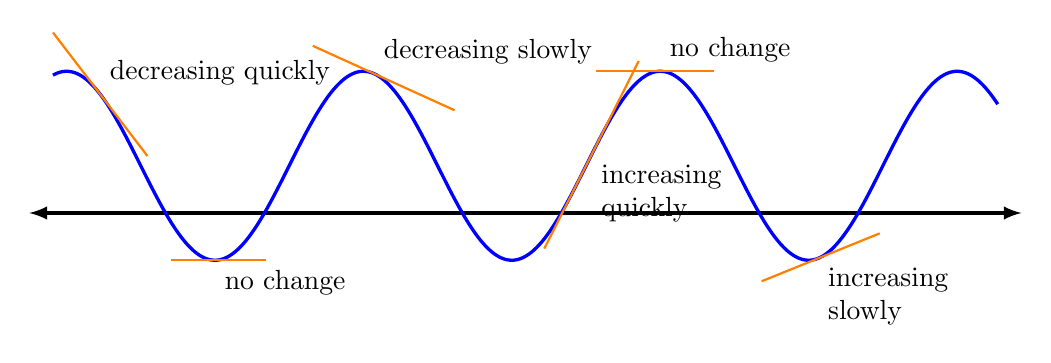
\begin{tikzpicture}[scale=0.6]
  \draw[latex-latex, very thick] (-5.5,0)--(15.5,0);

  \draw[domain=-5:15,samples=200,smooth,variable=\x, blue, very thick] plot ({\x},{1+2*sin(\x r)});
 
  \draw[domain=-5:-3,smooth,variable=\x, orange, thick] plot ({\x},{2*\x*cos(4 r) + 1 - 2*sin(4 r) + 8*cos(4 r)});
  \node[above right] at (-4,{1+2*sin(-4 r)}) {decreasing quickly};
 
  \draw[domain=-2.5:-.5,smooth,variable=\x, orange, thick] plot ({\x},{1+2*sin(-1.57 r)});
  \node[below right] at (-1.57,{1+2*sin(-1.57 r)}) {no change};
 
  \draw[domain=0.5:3.5,smooth,variable=\x, orange, thick] plot ({\x},{3.76562-0.4544*\x});
  \node[above right] at (1.8,{1+2*sin(1.8 r)}) {decreasing slowly};
 
  \draw[domain=5.4:7.4,smooth,variable=\x, orange, thick] plot ({\x},{1.98637*\x - 11.4797});
  \node[below right,text width=2cm] at (6.4,{1+2*sin(6.4 r)}) {increasing quickly};
 
  \draw[domain=6.5:9,smooth,variable=\x, orange, thick] plot ({\x},{1+2*sin(7.85 r)});
  \node[above right] at (7.85,{1+2*sin(7.85 r)}) {no change};
 
  \draw[domain=10:12.5,smooth,variable=\x, orange, thick] plot ({\x},{0.40601*\x - 5.50566});
  \node[below right,text width=2cm] at (11.2,{1+2*sin(11.2 r)}) {increasing slowly};
\end{tikzpicture}
Up until now, we have talked about needing two points to determine the slope of a line. However, as we begin talking about derivatives, we need to talk about the slope of a curve at a certain point. \\
Suppose that we wish to determine the slope of the curve $y=f(x)$ at the point where $x=a$. This is the same as finding the slope of the line tangent to the curve $y=f(x)$ at $x=a$.\\
When $x=a$, $y=f(x)$.  Therefore, we will be trying to determine the slope of the curve $y=f(x)$ at the point $(a, f(a))$.

\begin{center}
    
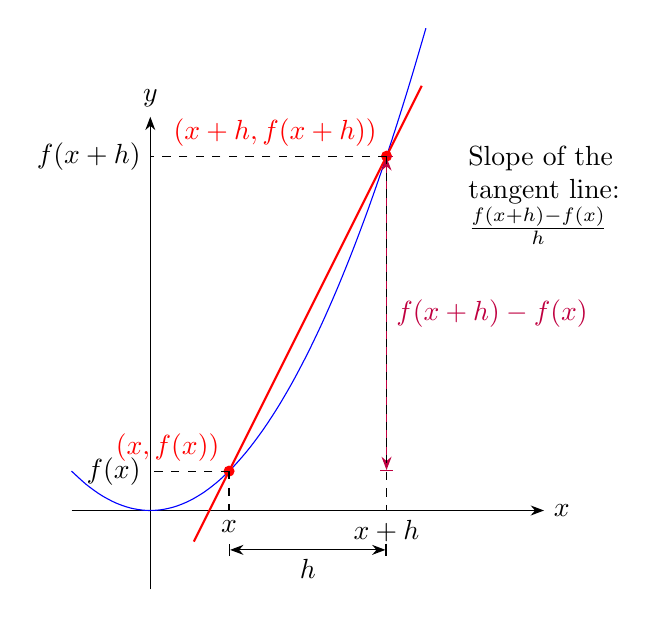
\begin{tikzpicture}[>=Stealth]
  \draw[->] (-1,0) -- (5,0) node[right] {$x$};
  \draw[->] (0,-1) -- (0,5) node[above] {$y$};
  
  \draw[scale=1,domain=-1:3.5,smooth,variable=\x,blue] plot ({\x},{0.5*\x*\x});
  
  \fill[red] (1,{0.5*1*1}) circle (2pt) node[above left] {$(x, f(x))$};
  \fill[red] (3,{0.5*3*3}) circle (2pt) node[above left] {$(x+h, f(x+h))$};
  
  \draw[red, thick, shorten <=-1cm,shorten >=-1cm] (1,{0.5*1*1}) -- (3,{0.5*3*3});
  
  \draw[|<->|] (1,-0.5) -- node[below] {$h$} (3,-0.5);
  
  \draw[|<->|,purple] (3,{0.5*3*3}) -- node[right] {$f(x+h)-f(x)$} (3,{0.5*1*1});
  
  \draw[dashed] (1,{0.5*1*1}) -- (1,0) node[below] {$x$};
  \draw[dashed] (3,{0.5*3*3}) -- (3,0) node[below] {$x+h$};
  \draw[dashed] (3,{0.5*3*3}) -- (0,{0.5*3*3}) node[left] {$f(x+h)$};
  \draw[dashed] (1,{0.5*1*1}) -- (0,{0.5*1*1}) node[left] {$f(x)$};

  \node at (5,4) [align=left] {Slope of the \\ tangent line:\\ $\frac{f(x+h)-f(x)}{h}$};
  
\end{tikzpicture}
\end{center}
    
\begin{tcolorbox}[colback=Orchid!5!white,colframe=Orchid!75!white,coltitle=white,title=Slope of Tangent ]
The derivative of the function $y=f(x)$ is given formula
  \[
  f'(x)=\lim_{h \to 0} \frac{f(x+h)-f(x)}{h},
  \]
 Other symbols for the derivative include $y'$ and $\frac{\delta y}{\delta x}$
\end{tcolorbox}
The derivative of a function allows you to determine the slope of the line tangent to a curve at a given point. In other words, you can find the slope of the line when you only know one point on the line. The value of the derivative is often called the instantaneous rate of change.
\subsubsection*{Example:}
Determine the derivative of the function $y=x^2$ and evaluate the derivative at the point where $x=3$.\\ \\ 
\textbf{Solution:}
\begin{align*}
    y' &= \lim_{x \to 0} \frac{f(x+h)-f(x)}{h}\\
    &= \lim_{h \to 0} \frac{(x+h)^2-x^2}{h}\\
    &= \lim_{h \to 0} \frac{x^2+2xh+h^2-x^2}{h}\\
    &= \lim_{h \to 0} \frac{2xh+h^2}{h}\\
    &= \lim_{h \to 0} (2x+h)\\
    &= 2x + 0\\
    &= 2x.\\
    & \therefore y'=2x, \text{ at } x=3. \\
    y' &=2(3)=6 
\end{align*}
By evaluating the limit as the change in \( x \) approaches zero, we find the derivative \( y' = 2x \). Therefore, at \( x = 3 \), the derivative equals 6.
\newpage
\subsubsection*{Example:}
Determine the equation of the tangent line to the curve $y=x^2$ at the point where $x=3$. \\ \\ 
\textbf{Solution:}
\begin{align*}
    y &= mx + b, \quad \text{we know } m = 6 \\
    y &= 6x + b \\
    & \text{Substitute }(3, 9): \\
    9 &= 6(3) + b \\
    -9 &= b \\
\end{align*}
Therefore, the equation of the tangent at \(x = 3\) is \(y = 6x - 9\).
\subsubsection*{Example:}
Give that $y=3x^2-7x+6$, determine the value of $\frac{\delta y}{\delta x}$ at $x=5$. \\ \\ 
\textbf{Solution:}
\begin{align*}
    f'(x)&=\lim_{h to 0} \frac{f(x+h)-f(x)}{h}\\
    &=\lim_{h to 0} \frac{3(x+h)^2-7(x+h)+6-(3x^2-7x+6)}{h}\\
    &=\lim_{h to 0} \frac{3(x^2+2xh+h^2)-7x+7h+6-3x^2+7x-6}{h}\\
    &=\lim_{h to 0} \frac{\cancel{3x^2}+6xh+3h^2\cancel{-7x}+7h\cancel{+6}\cancel{-3x^2}\cancel{+7x}\cancel{-6}}{h}\\
    &= \lim_{h to 0} \frac{6hx+3h^2-7h}{h}\\
    &= \lim_{h to 0} \frac{\cancel{h}(6x+3h-7)}{\cancel{h}}\\
    &=6x+3(0)-7\\
    &= 6x-7
\end{align*}
At $x=5$ 
\begin{align*}
    &\frac{\delta y}{\delta x}=6(5)-7\\
    &=23
\end{align*}
\newpage
\subsubsection*{Example:}
Determine the equation of the tangent line of the curve $f(x)= \frac{1}{x}$ at the point where $x=2$.\\ \\ 
\textbf{Solution:}
\begin{align*}
    f'(x) &=\lim_{h \to 0}\frac{f(x+h)-f(x)}{h}\\
    &=\lim_{h \to 0}\frac{\frac{1}{x+h}-\frac{1}{x}}{h}\\
    &=\lim_{h \to 0} \frac{\frac{x}{x(x+h)} -\frac{(x+h)}{x(x+h)}}{h}\\
    &=\lim_{h \to 0} \frac{x-(x+h)}{xh(x+h)}\\
    &=\lim_{h \to 0} \frac{x-x-h}{xh(x+h)}\\
    &=\lim_{h \to 0} \frac{\cancel{h}}{x\cancel{h}(x+h)}\\
    &=\frac{-1}{x(x+0)}\\
    &=\frac{-1}{x^2}
\end{align*}
At $x=3$, $y=\frac{1}{2}$. Therefore, the point is $\left(2,\frac{1}{2}\right)$.\\
The derivative is $\frac{-1}{x^2}$. Therefore, the slope at $x=2$ is $\frac{-1}{2^2}=\frac{-1}{4}$
\begin{align*}
    &= y=mx+b\\
    &= y=\frac{-1}{4}x+b\\
    & \text{Sub in} \left(2,\frac{1}{2}\right)\\
    \frac{1}{2} &= \frac{-1}{4}(2)+b\\
    1 &=b
\end{align*}
The equation of the tangent line is $y=-\frac{1}{4}x+1$
\newpage 
\subsubsection*{Example:}
Determine an equation of the line that is perpendicular to the tangent to the graph of $f(x)=\frac{1}{x}$ at the point where $x=2$ and that intersects it at the point of tangency.(this is called the normal) \\  \\ 
\textbf{Solution:}

Our point is still $\left(2,\frac{1}{2}\right)$, our perpendicular slope is the negative reciprocal of the $-1\frac{1}{4}$, which is 4.
\begin{align*}
    &\therefore y=4x+b\\
    &\text{sub in} \left(2,\frac{1}{2}\right)\\
    \frac{1}{2}&=4(2)+b\\
    \frac{-15}{2}&=b\\
\end{align*}
The equation of the normal is $y=4x-\frac{15}{2}$
\subsection*{The Existence of Derivatives:}
A function $f$ is said to be differentiable at $x=a$ if $f'(a)$ exists. At points where $f$ is not differentiable, we say that the derivative does not exist. Common ways for a derivative to not exist are shown.

\begin{figure}[h]
\centering
\begin{minipage}[b]{0.5\textwidth}
\centering
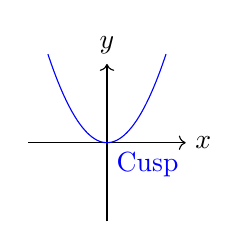
\begin{tikzpicture}[scale=0.5]
  % Cusp
  \draw[->] (-2,0) -- (2,0) node[right] {$x$};
  \draw[->] (0,-2) -- (0,2) node[above] {$y$};
  \draw[domain=-1.5:1.5, smooth, variable=\x, blue] plot ({\x}, {\x*\x});
  \node[below right, blue] at (0,0) {Cusp};
\end{tikzpicture}
\end{minipage}%
\begin{minipage}[b]{0.5\textwidth}
\centering
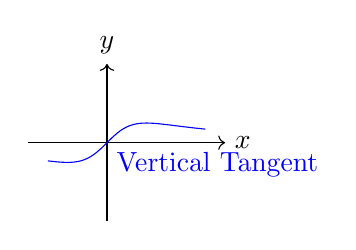
\begin{tikzpicture}[scale=0.5]
  % Vertical tangent
  \draw[->] (-2,0) -- (3,0) node[right] {$x$};
  \draw[->] (0,-2) -- (0,2) node[above] {$y$};
  \draw[domain=-1.5:2.5, smooth, variable=\x, blue] plot ({\x}, {\x/(1+\x*\x)});
  \node[below right, blue] at (0,0) {Vertical Tangent};
\end{tikzpicture}
\end{minipage}\\[20pt]
\begin{minipage}[b]{0.5\textwidth}
\centering
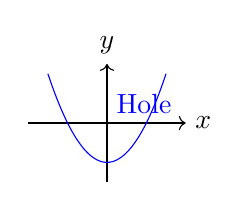
\begin{tikzpicture}[scale=0.5]
  % Hole
  \draw[->] (-2,0) -- (2,0) node[right] {$x$};
  \draw[->] (0,-1.5) -- (0,1.5) node[above] {$y$};
  \draw[domain=-1.5:1.5, smooth, variable=\x, blue] plot ({\x}, {(\x-1)*(\x+1)});
  \node[above right, blue] at (0,0) {Hole};
\end{tikzpicture}
\end{minipage}%
\begin{minipage}[b]{0.5\textwidth}
\centering
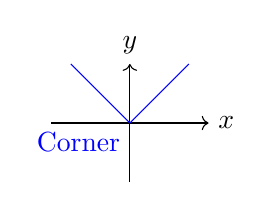
\begin{tikzpicture}[scale=0.5]
  % Corner
  \draw[->] (-2,0) -- (2,0) node[right] {$x$};
  \draw[->] (0,-1.5) -- (0,1.5) node[above] {$y$};
  \draw[domain=-1.5:1.5, variable=\x, blue] plot ({\x}, {abs(\x)});
  \node[below left, blue] at (0,0) {Corner};
\end{tikzpicture}
\end{minipage} 
\caption{Different Types of Discontinuities}
\label{fig:discontinuities}
\end{figure}


\section*{No Derivative}
\begin{minipage}[h]{0.7\textwidth}
  \centering
  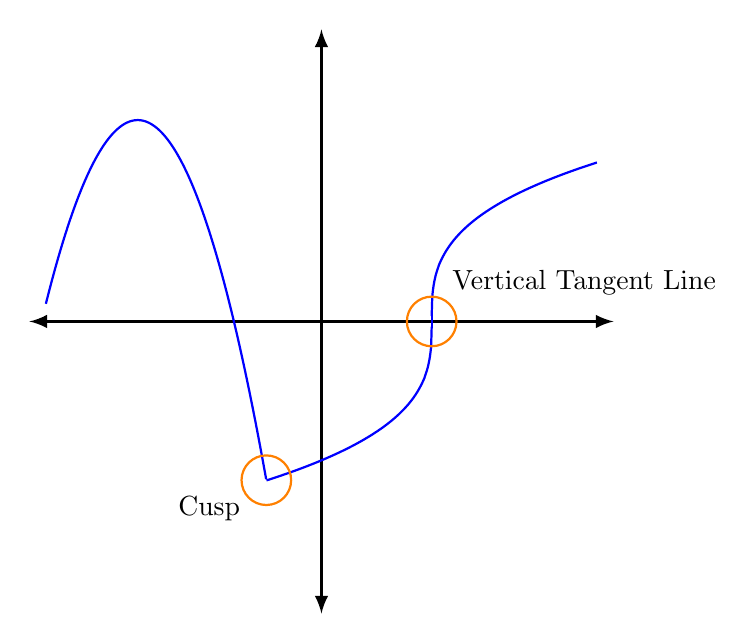
\begin{tikzpicture}[scale=0.7]
    \draw[latex-latex, very thick] (-5.3,0)--(5.3,0);
    \draw[latex-latex, very thick] (0,-5.3)--(0,5.3);
  
    \draw[domain=2.0001:5,samples=300,smooth,variable=\x, blue,  thick] plot ({\x},{2*exp(ln(\x-2)/3)});
    \draw[domain=2.0001:5,samples=300,smooth,variable=\x, blue,  thick,rotate around={180:(2,0)}] plot ({\x},{2*exp(ln(\x-2)/3)});
    \draw[blue,thick] (2,-0.1)--(2,0.1);
    \draw[domain=-5:-1,samples=300,smooth,variable=\x, blue,  thick] plot ({\x},-1.2*\x*\x-8*\x-9.68);
    \draw[orange,thick](-1,-2.88) circle (0.45);
    \draw[orange,thick](2,0) circle (0.45);
    \node[left] at (-1.3,-3.4) {Cusp};
    \node[above right] at (2.2,0.3) {Vertical Tangent Line};
  \end{tikzpicture}
\end{minipage}%
\begin{minipage}[t]{0.5\textwidth}
This graph represents a function that is not differentiable at certain points. The presence of a cusp and vertical tangent lines indicates that the function lacks a derivative at those points.
\end{minipage}

\section*{Inverse Derivative}
\begin{minipage}[h]{0.7\textwidth}
  \centering
  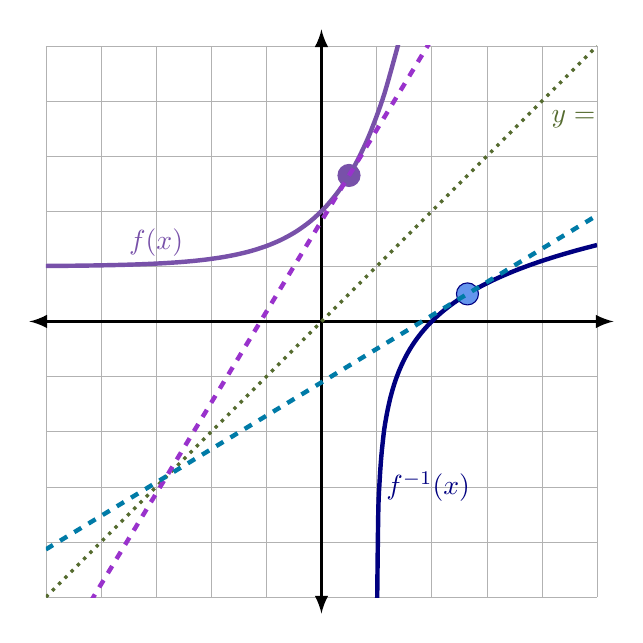
\begin{tikzpicture}[scale=0.7]
    \draw[black!30!white, very thin] (-5,-5) grid (5,5);
    \draw[latex-latex, very thick] (-5.3,0)--(5.3,0);
    \draw[latex-latex, very thick] (0,-5.3)--(0,5.3);
    
    \begin{scope}
        \clip (-5,-5) rectangle (5,5);
        \draw[very thick, OliveGreen,dotted](-5,-5)--(5,5);
        \node[OliveGreen,below right] at (4,4) {$y=x$};
        
        \draw[domain=-5:1.4,smooth,variable=\x, RoyalPurple, ultra thick] plot ({\x},{exp(\x)+1});
        \node[RoyalPurple,above] at (-3,1) {$f(x)$};
        \draw[RoyalPurple,fill=RoyalPurple] (0.5,2.649) circle [radius=0.2];
        \draw[domain=-4.5:2,smooth,variable=\x, DarkOrchid, ultra thick,dashed] plot ({\x},{1.649*\x+1.824});
        
        \draw[domain=1.003:5,smooth,variable=\x, NavyBlue, ultra thick, samples=150] plot ({\x},{ln(\x-1)});
        \node[NavyBlue,right] at (1,-3) {$f^{-1}(x)$};
        \draw[NavyBlue,fill=CornflowerBlue] (2.649,0.5) circle [radius=0.2];
        \draw[domain=-5:5,smooth,variable=\x, Cerulean, ultra thick,dashed] plot ({\x},{0.606*\x-1.105});
    \end{scope}
  \end{tikzpicture}
\end{minipage}%
  \vspace{2em}
\begin{minipage}[h]{0.5\textwidth}
This graph represents the inverse function of a function that has a derivative. The presence of a straight line indicates that the inverse function is linear. Additionally, the graph illustrates that the inverse function reverses the behavior of the original function with respect to the line $y=x$.
\end{minipage}



\subsection{Power Rule}
\begin{tcolorbox}[sharp corners=uphill,
    colback=purple!50!white,colframe=blue!25!black,coltext=yellow,
    fontupper=\Large\bfseries,arc=6mm,boxrule=2mm,boxsep=5mm]
  if $f(x)=x^{n}$, then $f'(x)=nx^{n-1}$
\end{tcolorbox}
  \textit{Proof}\\
  \begin{align*}
    f'(x)&=\lim_{h \to 0}\frac{f(x+h)-f(x)}{h}\\
    & \text{if } f(x)=x^n\\
    & \text{Then, } f(x+h)= (x+h)^n 
  \end{align*}
\subsubsection*{Example:}
if $f(x)= 4x^5$, then determine $f'(x)$. \\ \\ 
\textbf{Solution:}
\begin{align*}
    &= 4x^5\\
    &= (5)(4)x^{5-1}\\
    &=20x^4
\end{align*}
\subsubsection*{Example:}
if $f(x)= 11x^{\frac{5}{2}}$, then determine $f'(x)$.\\ \\ 
\textbf{Solution:}
\begin{align*}
    &= 11x^{\frac{5}{2}}\\
    &= \left(\frac{5}{2}\right)(10)x^{\frac{5}{2}-1}\\
    &= \frac{55}{2}x^{\frac{3}{2}}\\
\end{align*}
\subsubsection*{Example:}
if $f(x)=7x$, then determine $f'(x)$.\\ \\ 
\textbf{Solution:}
\begin{align*}
    &=(0)(7)x^{0-1}\\
    &=0
\end{align*}
\newpage
\subsection{Product Rule}
\begin{tcolorbox}[colback=Orchid!5!snow, colframe=nadeshikopink!50!white,
  colbacktitle=mordantred19!75!mistyrose, title=Product Rule]

The product rule states that if $p(x)=f(x)g(x)$, then\\ $p'(x)=f'(x)g(x)+f(x)g'(x)$.
\textbf{Product Rule in Newton Notation.}\\


$\frac{\delta}{\delta x}(uv)=\left(\frac{\delta u}{\delta x}\right)v+u\left(\frac{\delta v}{\delta x}\right)$
\textbf{Product Rule in Leibniz Notation}

\end{tcolorbox}
\textit{Proof of the Product Rule}
\begin{align*}
    p'(x) &= \lim_{h \to 0}\frac{p(x+h)-p(x)}{h}\\
    &=\lim_{h \to 0}\frac{f(x+h)g(x+h)-f(x)g(x)}{h}\\
    &=\lim_{h \to 0}\frac{f(x+h)g(x+h)\textcolor{red}{-f(x)g(x+h)+f(x)g(x+h)}-f(x)g(x)}{h}\\
    &= \lim_{h \to 0}\left[\frac{f(x+h)-f(x)}{h}\right]g(x+h)+f(x)\left[\frac{g(x+h)-g(x)}{h} \right]\\
    &=\left(\lim_{h \to 0} \frac{f(x+h)-f(x)}{h} \right) \left[\lim_{h \to 0}g(x+h)\right]+\left[\lim_{h \to 0} f(x)\right]\left(\lim_{h \to 0}\frac{g(x+h)-g(x)}{h}  \right)\\
    &=f'(x)g(x)+f(x)g'(x)
\end{align*}
\subsection*{Example}
Differentiate $h(x)=(x^3-2x)(3x^4+2x+8)$.\\
\textbf{Solution:}
$h'(x)=(3x^2-2)(3x^4+2x+8)+(x^3-2x)(12x^3+2)$.

Because of the power rule, we are able to say that the derivative of $kf(x)$ where is a scalar is $kf'(x)$.  In other words, we are able to just leave the scalar alone in front and determine the derivative of the function.\\
An example of this would be that if $y=7(3x^2+2x+6)$, then $$\frac{\delta y}{\delta x}=7(6x+2)$$\\
In other words, the derivative would equal 7 times the derivative of the polynomial.\\
How do we know this? By the power rule. Here’s the explanation.
Let $f(x)g(x)$, where $f(x)=7$ and $g(x)=3x^2+2x+6$.  

\begin{align}
    \frac{\delta y}{\delta x}&=f'(x)g(x)+f(x)g'(x)\\
    \frac{\delta y}{\delta x}&=(0)(3x^2+2x+6)+7(6x+2)\\
    &=7(6x+2)
\end{align}

\subsection{Quotient Rule}
"Low di high minus high di low over low low." \\
What does this mean? Well it means the quotient rule

\begin{tcolorbox}[colback=blue!5!snow, colframe=white!50!white,
  colbacktitle=blue!75!mistyrose, title=Quotient Rule]
if $h(x)=\frac{f(x)}{g(x)}$, then $h'(x)=\frac{f'(x)g(x)-f(x)g'(x)}{[g(x)]^2}, g \neq 0$\\
In Leibniz notation, $\frac{\delta }{\delta x}(\frac{u}{v})=\frac{\frac{\delta u}{\delta x}v- u\frac{\delta v}{\delta x}}{v^2}$
\end{tcolorbox}
\textit{Proof:}
\begin{align*}
    h(x)&=\frac{f(x)}{g(x)} \implies h(x)g(x)=f(x)\\
    & \therefore \text{by the product rule, } h'(x)g(x)+h(x)g'(x)=f(x)'\\
    &\implies h'(x)\cancel{g(x)}=\frac{f'(x)-h(x)g'(x)}{g(x)}\\
    &h'(x)=\frac{f'(x)-\left[\frac{f(x)}{g(x)}\right]g'(x)}{g(x)}\\
    &=\frac{f'(x)\left( \textcolor{red}{\frac{g(x)}{g(x)}}\right)-\frac{f(x)g'(x)}{g(x)}}{g(x)}\\
    &=\frac{\frac{f'(x)g(x)}{g(x)}-\frac{f(x)g'(x)}{g(x)}}{g(x)}\\
    &=\frac{f'(x)g(x)-f(x)g'(x)}{[g(x)]^2}
\end{align*}
\subsubsection*{Example:}
Determine the derivative of $h(x)=\frac{3x-4}{x^2+5}$.\\
\textbf{Solution:}
$h'(x)=\frac{(x^2+5)(3)-(3x+4)(4)}{(x^2+5)^ 2}$
\newpage 


\subsection{Chain Rule}
\begin{tcolorbox}[colback=OliveGreen!5!snow, colframe=white!50!white,
  colbacktitle=OliveGreen!75!mistyrose, title=Chain Rule]
The chain rule states 
if $h(x)=f \circ g(x)$, then $f'(g(x))g'(x)$ \\
$\frac{\delta y}{\delta x}=\frac{\delta y}{\delta u} \times \frac{\delta u}{\delta x}$
\end{tcolorbox}
\textit{Proof:}\\
\begin{align*}
\left[f(g(x)) \right]'&=\lim_{h \to 0} \frac{f(g(x+h)-f(g(x)))}{h}\\
&= \lim_{h \to 0} \left[ \frac{f(g(x+h)-f(g(x))}{\textcolor{red}{g(x+h)-g(x)}} \frac{\textcolor{red}{g(x+h)-g(x)}}{h}\right]\\
&=\lim_{h \to 0}\frac{f(g(x+h))-f(g(x))}{g(x+h)-g(x)} \lim_{h \to 0}\frac{g(x+h)-g(x)}{h}\\
&\boxed{\text{let k } = g(x+h)-g(x) \therefore \text{ as } h \to 0, k \to0}\\
&= \left[\lim_{\textcolor{red}{k \to 0}}\frac{f(g(x+\textcolor{red}{k})-f(g(x))}{\textcolor{red}{k}} \right]\left[ \lim_{h \to 0}\frac{g(x+h)-g(x)}{h}\right]\\
&=f'(g(x))g'(x)
\end{align*}
\subsubsection*{Example 1:}
Determine the derivative of $h(x)=(10x^3-7x^2+3x-9)^{14}$\\
\textbf{Solution:}
$h'(x)=14(10x^3-7x^2+3x-9)^{13}(30x^2-14x+3)$
\subsubsection*{Example 2:}
Suppose $f(12)=-7, g(3)=12, f'(12)=11$ and $g'(3)=9$. If $h(x)=f(g(x))$, then evaluate $h'(3)$.\\
\textbf{Solution:}
\begin{align*}
    h'(x)&=f(g(x))\\
    h'(3)&=f'(g(3))g(3)\\
    &=f'(12)(9)\\
    &=(11)(9)\\
    &=99
\end{align*}
\newpage 

\subsection{Derivatives Not in Terms of x:}
Every time that we state a rate of change, we state that rate of change with respect to something.\\
For instance, if we talk about speed, we are talking about distance with respect to time.\\
When we discuss slope on a Cartesian plane, we use the formula:
$$m=\frac{y_2-y_1}{x_2-x_1}$$
In other words, we talk about the change in y with respect x.\\
Similarly, when we determine a derivative(which is just an instantaneous rate of change, or slope at a point), we determine the derivative with respect to something. Usually, we derivative with respect to x. However, this isn't always case.\\

The definition of a derivative is 
$$f'(x)=\lim_{h \to 0}\frac{f(x+h)-f(x)}{h}$$
The derivative is the limit of the slope between two points on a relation as those two points get infinitely close together. Alternatively, then we could define the derivative $$f'(x)= \lim_{x \to a }\frac{f(x)-f(a)}{x-a}$$

\subsubsection*{Example 1:}
Suppose $y=3(2x^2+x+-1)^4$. Determine $\frac{\delta y}{\delta x}$.\\
\textbf{Solution:}
$\frac{\delta y}{\delta x}=12(2x^2+x-1)^3(4x+1)$
\subsubsection*{Example 2:}
Suppose $y=3(2x^3+x-1)^4$. Determine $\frac{\delta y}{d(2x^2+x-1)}$.\\
\textbf{Solution:}
\begin{align*}
    \text{ let w } &= (2x^2+x-1)^4\\
    y&=3w^4\\
    \frac{\delta y}{\delta x}&=12w^3\\
    \frac{\delta y}{d(2x^2+x-1)}&=12(2x^2+x-1)^3
\end{align*}

\begin{center}
\begin{figure}
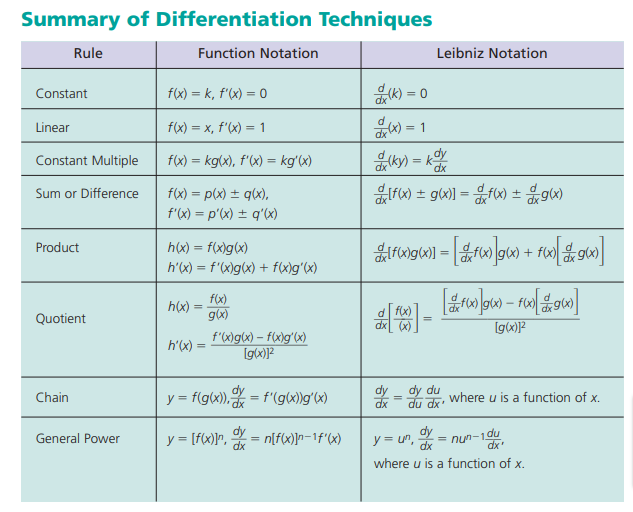
\includegraphics[width=1\textwidth]{imgs/summary of differentiation techniques.png}
\caption{Summary of Differentiation Techniques }
\end{figure}
\end{center}
\newpage 


\subsection{Implicit Differentiation}
Unit now, we have been determining derivatives when y is stated explicitly in terms of x.\\
However, sometimes are equation in terms of x, and remember to use the chain rule when differentiating terms containing y.\\
We may need to use other rules of differentiation as well.\\
\subsubsection{Intro to How Implicit Differentiation Works:}
\begin{itemize}
    \item The derivative pf $5x^3$ with respect to x is $15x^2$. We can think of this slightly differently though and say that the derivative of $5x^3$ with respect to x is $15x^2 \frac{\delta x}{\delta x}$ and that since $\frac{\delta x}{\delta x}=1$, therefore the derivative of $5x^3$ with respect to is $15x^2$
    \item By the same way of thinking, the derivative of $5y^3$ with respect to x is $15y^2 \frac{\delta y}{\delta x}$
\end{itemize}
\subsubsection*{Example}
If $x^2+y^2=25$, determine $\frac{\delta y}{\delta x}$ and determine the slope of the tangent to the curve at the point (3,-4).
\begin{align*}
    2x+2y \frac{\delta y}{\delta x}&=0\\
    2y \frac{\delta y}{\delta x}&=-2x\\
    \frac{\delta y}{\delta x}=\frac{-2x}{2y}\\
    \frac{\delta y}{\delta x}=\frac{-x}{y}\\
    \text{at }(3,-4), \frac{\delta y}{\delta x}&=\frac{-3}{-4}\\
    \frac{\delta y}{\delta x}=\frac{3}{4}
\end{align*}

\newpage 
\subsection{Related Rates}

\begin{itemize}
    \item After 1 second, the circular ripple would have an area of $\pi(1)^2=\pi m^2$ 
    \item After 2 seconds, the circular ripple would have an area of $\pi(2)^2=4\pi m^2$ (an increase of $3\pi m^2$)
    \item After 3 seconds, the circular ripple would have an area of $\pi(3)^2=9\pi m^2$ (an increase of $5\pi m^2$)
    \item After 4 seconds, the circular ripple would have an area of $\pi(4)^2=16\pi m^2$ (an increase of $7\pi m^2$)
\end{itemize}

We see that although the rate of increase of the radius remains constant, the rate of increase of the area is changing. The rate of increase of the area is related to the rate of increase of the radius. We call it a “related rate”. The rate of increase of the area is a function of time and it is not a constant.

Examples of Related Rates in Calculus
There are many types of related rates in Calculus. For example,
\begin{itemize}

\item Imagine a stone in a pond causing a circular ripple. The rate of increase of the area of the circular ripple will be related to the rate of increase of the radius of the ripple. If the rate of increase of the radius of the circular ripple is constant, the rate of increase of the area of the circular ripple will not be.

\item Imagine blowing air into a spherical balloon. The rate of increase of the radius of the sphere will be related to the rate of increase of the volume of the sphere. If the rate of increase of the volume of air in the sphere is constant, the rate of increase of the radius of the sphere will not be.

\item Imagine filling a cone shaped container with liquid. The rate of increase of the height of the liquid will be related to the rate of increase of the volume of the liquid in the cone. If the rate of increase of the volume of the liquid is constant, the rate of increase of the height of the liquid will not be.

There are many more examples.

\end{itemize}
\subsubsection{How To Approach a Related Rates Problem}
\begin{enumerate}
\item Some people like to draw a diagram.

\item Assign a variable to each quantity in the problem that is a function of the independent variable.  (We’ll assume for the remainder of this discussion that the independent variable is time)

\item Develop an equation that associates the variables with one another.4.Differentiate (possibly using implicit differentiation).

\item Substitute in given information and solve for the required rate of change.
\end{enumerate}
\subsubsection*{Example:} 
When a raindrop falls into a small puddle, it creates a circular ripple that spreads out from the point where the raundrop hit. The radius of the circle grows at a rate of 3 cm/s.
a) determine the rate of increase of the circumference of the circle with respect to time.\\
b) determine the rate of increase \\
\textbf{Solution:}

a) 
\begin{align*}
    \frac{\delta r}{dt}&=3\\
    C&=2\pi r\\
    \frac{\delta c }{\delta t}&=2 \pi \frac{\delta r}{\delta t}\\
    &=2 \pi (3cm/s)\\
    &=6 \pi cm/s 
\end{align*}
$\therefore$ the circumference increase at a rate of $6 \pi$ cm/s
b) 
\begin{align*}
    A&=\pi r^2\\
    \frac{\delta A}{\delta t} &=2\pi r \frac{\delta r}{\delta t}\\
    A&=81 \pi \\
    r^2&=81\\
    r&=9\\
    \frac{\delta A}{\delta t}&=2\pi (9 cm)(3cm/s)\\
    &=54\pi cm^2/s
\end{align*}
\textbf{Visit \href{https://openstax.org/books/calculus-volume-1/pages/4-1-related-rates}{here} for more examples.}

 
\subsubsection{How to approach each problem}
\begin{itemize}
    \item Identify the given variables and the quantities that need to be determined. Draw a picture if one is not given.

    \item Write an equation involving the rates whose variables are given or need to be determined. Do not substitute yet unless the value will never change.

    \item Using the chain rule, implicitly differentiate both sides of the equation with respect to time ($t$).

    \item Substitute into the resulting equation all known values for the variables and their rates of change. Then, solve for the required rate of change.	
\end{itemize}
	

\end{document}